\documentclass{beamer}
\usepackage{graphicx}
\usepackage{polski}
\usepackage[utf8]{inputenc}
\graphicspath{ {src/obrazy/} }
\usetheme{Warsaw}
\begin{document}
\title{Rozpoznawanie emocji w mowie}
\author{Wojciech Decker}
\maketitle
\begin{frame}
  \frametitle{Definicja emocji}
  emocje – świadome lub nieświadome silne, względnie nietrwałe, gwałtowne uczucia o silnym zabarwieniu i wyraźnym wartościowaniu, poprzedzone jakimś wydarzeniem i ukierunkowane. 
\end{frame}
\begin{frame}
  \frametitle{Jak człowiek okazuje emocje?}
  \begin{itemize}
    \item mimika
    \item gesty
    \item mowa ciała
    \item reakcje wewnętrzne organizmu
    \item mowa
  \end{itemize}
%https://www.newscientist.com/article/mg22129595-200-feeling-sad-computer-knows-by-looking-at-how-you-move/
\end{frame}
\begin{frame}
  \frametitle{Gdzie się stosuje?}
  \begin{itemize}
    \item nauka rozpoznawania emocji (autyzm)
    \item centra obsługi klienta
    \item rozpoznawanie stanu pacjentów
    \item komputer rozumie emocje człowieka
  \end{itemize}
\end{frame}
\begin{frame}
  \frametitle{Podstawowe emocje}
  \begin{itemize}
    \item radość
    \item smutek
    \item gniew
    \item strach
    \item zdziwienie
    \item zniesmaczenie
  \end{itemize}
\end{frame}
\begin{frame}
  \frametitle{Model Plutchika}
  \begin{itemize}
	\item radość – smutek
	\item złość – strach
	\item oczekiwanie – zaskoczenie
	\item zaufanie – zniesmaczenie
  \end{itemize}
\end{frame}
\begin{frame}
  \frametitle{Model Plutchika - obraz}
    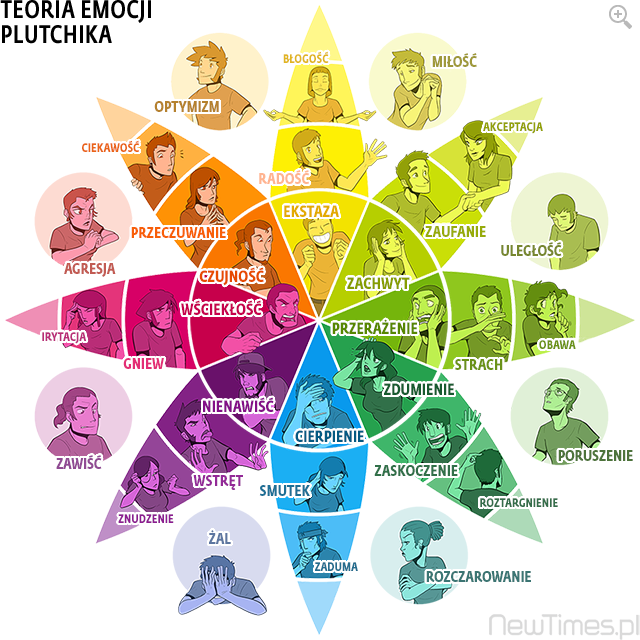
\includegraphics[scale=.4]{plutchik}
\end{frame}
\begin{frame}
  \frametitle{Dla czego mowa?}
  \begin{itemize}
    \item można ją nagrać wszędzie
    \item kamera musi być skierowana na człowieka
    \item twarz, ciało można zasłonić
    \item wystarczy mikrofon
  \end{itemize}
\end{frame}
\begin{frame}
  \frametitle{Różnice między mówcami}
  \begin{itemize}
    \item cechy indywidualne
    \item kultura
    \item środowisko
    \item cechy sygnału % różne cechy u różnych ludzi
  \end{itemize}
\end{frame}
\begin{frame}
  \frametitle{Emocje w przestrzeni dwuwymiarowej}
    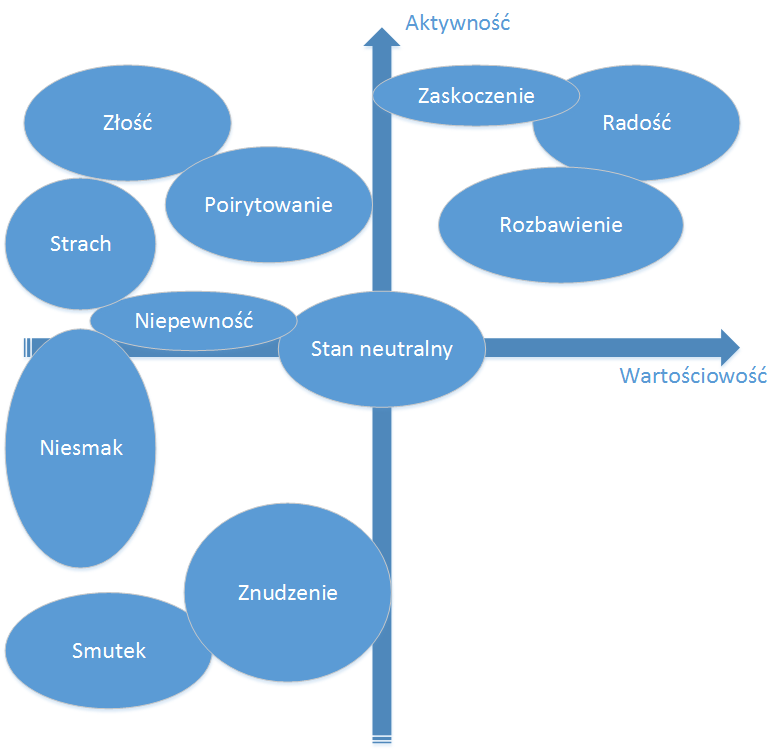
\includegraphics[scale=.25]{dwa_wymiary}
\end{frame}
\begin{frame}
  \frametitle{Klasyfikatory}
  \begin{itemize}
        \item k-najbliższych sąsiadów
	\item metodę drzewa
	\item analizę dyskryminacyjną
	\item ukryte modele Markowa
	\item gusowskie modele mieszane
	\item sztuczne sieci neuronowe
        \item maszynę wektorów wspierających
        \item podejście mieszane
  \end{itemize}
\end{frame}
\begin{frame}
  \frametitle{Bazy mowy}
  \begin{itemize}
    \item spontaniczne
    \item odgrywane
  \end{itemize}
\end{frame}
\end{document}
